\documentclass{../khlslides}


\title[Functies]{Functies}
\author{Fr\'ed\'eric Vogels}


\pgfkeys{/tikz/flowchart/node/.style={rectangle,fill=blue,opacity=0.5,text opacity=1,drop shadow,inner sep=2mm}}
\pgfkeys{/tikz/flowchart/arrow/.style={-latex,flowchart/arrowline}}
\pgfkeys{/tikz/flowchart/arrowline/.style={thick}}


\newcommand{\lcurly}{{\tt{\char '173}}}
\newcommand{\link}[2]{\href{#1}{\beamergotobutton{#2}}}
\newcommand{\PLACEHOLDER}[1]{\ensuremath{\langle}\textrm{\textit{#1}\ensuremath{\rangle}}}


\pgfkeys{
  /wof/sequence point/.cd,
  placement/.initial=above,
  rotation/.initial=0,
  /wof/sequence link/.cd,
  label/.initial={},
  /wof/round/.cd,
  name prefix/.initial=,
  /tikz/.cd,
  sequence point/.style={blue!50,thick,fill=white},
  sequence point label/.style={font=\tiny,black},
  sequence link/.style={blue!50,thick},
  active/.style={fill=red,thick,red}
}
\newcommand<>{\seqpoint}[3][]{
  \only#4{{
  \pgfkeys{/wof/sequence point/.cd,#1}
  \pgfkeys{/wof/sequence point/placement/.get=\placement}
  \pgfkeys{/wof/sequence point/rotation/.get=\rotation}
  \draw[sequence point] (#2) circle (.05)
                        node[sequence point label,\placement,rotate=\rotation] {#3};
}}}
\newcommand<>{\seqlink}[3][]{\only#4{{
  \pgfkeys{/wof/sequence link/.cd,#1}
  \pgfkeys{/wof/sequence link/label/.get=\seqlinklabel}
  \draw[sequence link] (#2) -- (#3) node[midway,sloped,yshift=1mm,font=\tiny,black] {\seqlinklabel};
}}}

\newcommand{\singleround}[1][]{{
}}


\begin{document}

\begin{frame}
  \titlepage
\end{frame}

% \begin{frame}
  \frametitle{Rad van Fortuin}
  \begin{center}
    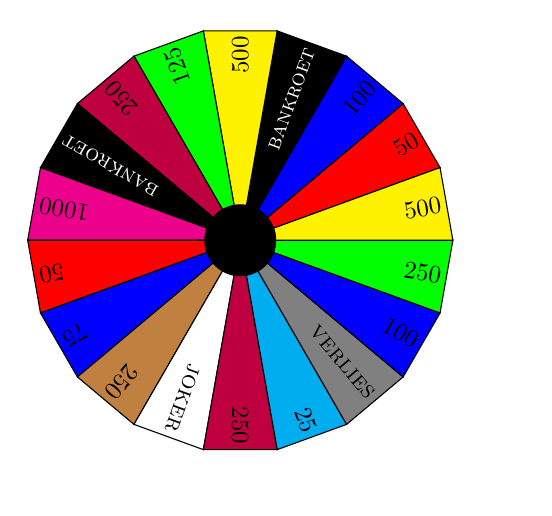
\begin{tikzpicture}[scale=.9,transform shape]
      \path[use as bounding box] (-3,-3.5) rectangle (4,3);

      \foreach[count=\i] \text/\c in {50/red,100/blue,{\color{white}\sc\small bankroet}/black,500/yellow,125/green,250/purple,{\color{white}\sc\small bankroet}/black,1000/magenta,50/red,75/blue,250/brown,{\sc joker}/white,250/purple,25/cyan,{\sc verlies}/gray,100/blue,250/green,500/yellow} {
        \pgfmathparse{20}\let\deltaangle\pgfmathresult
        \pgfmathparse{\i * \deltaangle}\let\startangle\pgfmathresult
        \pgfmathparse{\startangle + \deltaangle/2}\let\midangle\pgfmathresult
        \pgfmathparse{\startangle + \deltaangle}\let\endangle\pgfmathresult
        \draw[fill=\c] (0,0) -- (\startangle:3cm) -- (\endangle:3cm) -- cycle;
        \coordinate (cell \i) at (\midangle:3cm);
        \node[anchor=east,rotate=\midangle] at (\midangle:3cm) {\text};
      }
      \draw[fill=black] (0,0) circle (.5cm);
    \end{tikzpicture}
    \vskip4mm
    We herbezoeken hetzelfde voorbeeld
  \end{center}
\end{frame}



\begin{frame}
  \frametitle{Rad van Fortuin: E\'en Beurt}
  \begin{center}
    \begin{tikzpicture}
      \singleround
    \end{tikzpicture}
  \end{center}
\end{frame}

\begin{frame}
  \frametitle{Rad van Fortuin: Twee Beurten}
  \begin{center}
    \begin{tikzpicture}
      \begin{scope}[scale=0.5,transform shape]
        \singleround[name prefix=a]
      \end{scope}

      \begin{scope}[scale=0.5,transform shape,xshift=10cm]
        \singleround[name prefix=b]
      \end{scope}

      \draw[sequence link] (a exit) -- (b init);
    \end{tikzpicture}
  \end{center}
\end{frame}

\begin{frame}
  \frametitle{Rad van Fortuin: Drie Beurten}
  \begin{center}
    \begin{tikzpicture}
      \begin{scope}[scale=0.33,transform shape]
        \singleround[name prefix=a]
      \end{scope}

      \begin{scope}[scale=0.33,transform shape,xshift=10cm]
        \singleround[name prefix=b]
      \end{scope}

      \begin{scope}[scale=0.33,transform shape,xshift=20cm]
        \singleround[name prefix=c]
      \end{scope}

      \draw[sequence link] (a exit) -- (b init);
      \draw[sequence link] (b exit) -- (c init);
    \end{tikzpicture}
  \end{center}
\end{frame}

\begin{frame}
  \frametitle{Rad van Fortuin: 16 Beurten}
  \begin{center}
    \begin{tikzpicture}
      \begin{scope}[scale=0.20,transform shape]
        \singleround[name prefix=1]
      \end{scope}

      \begin{scope}[scale=0.20,transform shape,xshift=10cm]
        \singleround[name prefix=2]
      \end{scope}

      \begin{scope}[scale=0.20,transform shape,xshift=20cm]
        \singleround[name prefix=3]
      \end{scope}

      \begin{scope}[scale=0.20,transform shape,xshift=30cm]
        \singleround[name prefix=4]
      \end{scope}

      \begin{scope}[scale=0.20,transform shape,xshift=35cm,yshift=-6cm,rotate=180]
        \singleround[name prefix=5]
      \end{scope}

      \begin{scope}[scale=0.20,transform shape,xshift=25cm,yshift=-6cm,rotate=180]
        \singleround[name prefix=6]
      \end{scope}

      \begin{scope}[scale=0.20,transform shape,xshift=15cm,yshift=-6cm,rotate=180]
        \singleround[name prefix=7]
      \end{scope}

      \begin{scope}[scale=0.20,transform shape,xshift=5cm,yshift=-6cm,rotate=180]
        \singleround[name prefix=8]
      \end{scope}

      \begin{scope}[scale=0.20,transform shape,yshift=-15cm]
        \singleround[name prefix=9]
      \end{scope}

      \begin{scope}[scale=0.20,transform shape,xshift=10cm,yshift=-15cm]
        \singleround[name prefix=10]
      \end{scope}

      \begin{scope}[scale=0.20,transform shape,xshift=20cm,yshift=-15cm]
        \singleround[name prefix=11]
      \end{scope}

      \begin{scope}[scale=0.20,transform shape,xshift=30cm,yshift=-15cm]
        \singleround[name prefix=12]
      \end{scope}

      \begin{scope}[scale=0.20,transform shape,xshift=35cm,yshift=-21cm,rotate=180]
        \singleround[name prefix=13]
      \end{scope}

      \begin{scope}[scale=0.20,transform shape,xshift=25cm,yshift=-21cm,rotate=180]
        \singleround[name prefix=14]
      \end{scope}

      \begin{scope}[scale=0.20,transform shape,xshift=15cm,yshift=-21cm,rotate=180]
        \singleround[name prefix=15]
      \end{scope}

      \begin{scope}[scale=0.20,transform shape,xshift=5cm,yshift=-21cm,rotate=180]
        \singleround[name prefix=16]
      \end{scope}

      \foreach \i in {1,...,15} {
        \pgfmathparse{int(\i+1)}\let\j\pgfmathresult
        \draw[sequence link] (\i\space exit) |- (\j\space init);
      }
    \end{tikzpicture}
  \end{center}
\end{frame}

\begin{frame}
  \frametitle{Lus}
  \begin{center}
    \begin{tikzpicture}
      \path[use as bounding box] (0,-3) rectangle (8,4);
      \singleround[name prefix=b]
      \only<1-2>{
        \draw[sequence link,-latex,red] (b exit) -- +(0,-3) -| ($ (b init) + (0,-.2) $);
      }

      \only<3->{
        \draw[sequence link,-latex,red] (b exit) -- +(0,-3) node[midway,sloped,black,yshift=1mm,font=\tiny] {!spel gedaan} -| ($ (b init) + (0,-.2) $);
        \draw[sequence link,-latex,red] (b exit) -- +(2,0) node[midway,sloped,black,yshift=1mm,font=\tiny] {spel gedaan};
      }

      \only<2>{
        \node[opacity=.85,text opacity=1,fill=blue!50] (note) at (6,0) {\parbox{3cm}{\raggedright Lus laat toe berekeningen te herhalen}};
        \draw[-latex,blue!50,thick] (note) -- ($ (b exit) + (-0.1,-1) $);
      }

      \only<4>{
        \node[opacity=.85,text opacity=1,fill=blue!50] (note) at (8,2) {\parbox{3cm}{\raggedright Lus moet ooit eindigen}};
        \draw[-latex,blue!50,thick] (note) -- ($ (b exit) + (1,.2) $);
      }
    \end{tikzpicture}
  \end{center}
\end{frame}

%%% Local Variables: 
%%% mode: latex
%%% TeX-master: "loops"
%%% End: 

\begin{frame}
  \frametitle{Functies: Groeperen van Berekeningen}
  \begin{columns}
    \column{.5\linewidth}
    \code[width=.4\linewidth]{seq.js}
    \column{.5\linewidth}
    \code{seq2.js}
  \end{columns}
  \begin{tikzpicture}[overlay,remember picture]
    \only<2>{
      \foreach \from/\to in {a/b,b/c,c/d,d/e} {
        \draw[-latex] (\from1.east) to[bend left=30] (\to1.east);
      }

      \draw[-latex] (a2.east) to[bend left=30] (f2.east);
      \draw[-latex] (f2.west) to[bend left=30] (b2.west);
      \foreach \from/\to in {b/c,c/d,d/e} {
        \draw[-latex] (\from2.east) to[bend left=30] (\to2.east);
      }
    }
  \end{tikzpicture}
\end{frame}

\begin{frame}
  \frametitle{BMI}
  \code[font size=\small]{bmi.js}
\end{frame}

\begin{frame}
  \frametitle{BMI}
  \code[font size=\small]{bmi2.js}
  \begin{tikzpicture}[overlay,remember picture]
    \only<2>{
      \node[/khl/note,anchor=south west] (note bmi computation) at ($ (compute bmi) + (1,1.5) $) {Plaatst bmi in variabele {\tt bmi}};
      \draw[/khl/note arrow] (note bmi computation) |- (compute bmi);
      \draw[/khl/note arrow] (note bmi computation) |- (set bmi);
    }
    \only<3>{
      \node[/khl/note,anchor=south west] (note bmi evaluation) at ($ (compute bmi) + (1,1.5) $) {Plaatst string in variabele {\tt resultaat}};
      \draw[/khl/note arrow] (note bmi evaluation) |- (evaluate bmi);
      \draw[/khl/note arrow] (note bmi evaluation) |- (set result 1);
      \draw[/khl/note arrow] ($ (note bmi evaluation.north west) ! 0.75 ! (note bmi evaluation.north) $) |- (set result 2);
    }
  \end{tikzpicture}
\end{frame}

\begin{frame}
  \frametitle{BMI voor Twee Personen}
  \begin{center}
    \Huge Wat als we het BMI moeten uitrekenen van twee personen?
  \end{center}
\end{frame}

\begin{frame}
  \frametitle{BMI voor Twee Personen}
  \code[font size=\small]{bmi-2people.js}
  \begin{tikzpicture}[overlay,remember picture]
    \only<2>{
      \node[/khl/note] (note copy) at ($ (copy length) ! .5 ! (copy weight 2) + (5,0) $) {
        \parbox{6cm}{\raggedright
          {\tt berekenBMI()} verwacht waarden in {\tt gewicht} en {\tt lengte}
        }        
      };

      \draw[/khl/note arrow] (note copy.north) |- (copy weight);
      \draw[/khl/note arrow] ($ (note copy.north west) ! .75 ! (note copy.north) $) |- (copy length);
      \draw[/khl/note arrow] ($ (note copy.south west) ! .75 ! (note copy.south) $) |- (copy weight 2);
      \draw[/khl/note arrow] (note copy.south) |- (copy length 2);
    }

    \only<3>{
      \node[/khl/note] (note bmi) at ($ (copy bmi) ! .5 ! (copy bmi 2) + (3,0) $) {
        \parbox{6.5cm}{\raggedright
          {\tt berekenBMI()} plaatst resultaat in {\tt bmi}
        }        
      };

      \draw[/khl/note arrow] (note bmi.north) |- (copy bmi);
      \draw[/khl/note arrow] (note bmi.south) |- (copy bmi 2);
    }
  \end{tikzpicture}
\end{frame}

%%% Local Variables: 
%%% mode: latex
%%% TeX-master: "functions"
%%% End: 

\begin{frame}
  \frametitle{BMI Berekening: Inputs en Outputs}
  \begin{center}
    \begin{tikzpicture}
      \path[use as bounding box] (-1,-1) rectangle (1,1);
      \node[minimum width=4cm,minimum height=1cm,fill=green!25,drop shadow] (bmi) {\tt berekenBMI()};
      \draw[-latex] ($ (bmi.west) ! .5 ! (bmi.north west) $) +(-2,0) -- +(0,0)
                    node[midway,above,font=\small] {lengte};
      \draw[-latex] ($ (bmi.west) ! .5 ! (bmi.south west) $) +(-2,0) -- +(0,0)
                    node[midway,below,font=\small] {gewicht};
      \draw[-latex] (bmi.east) -- +(2,0)
                    node[midway,below,font=\small] {bmi};
    \end{tikzpicture}
    \vskip5mm
    \visible<2>{We focussen op de inputs}
  \end{center}
\end{frame}

\begin{frame}
  \frametitle{Parameters}
  \begin{itemize}
    \item Functies kunnen \emph{parameters} hebben
    \item Vermelden expliciet welke inputs een functie nodig heeft
    \item BMI parameters: gewicht en lengte
  \end{itemize}
  \code[font size=\small]{bmi-params.js}
\end{frame}

{
  \newcommand{\CODE}[9]{
    \def\paramx{#1}
    \def\paramy{#2}
    \def\paramz{#3}
    \def\localx{#4}
    \def\localy{#5}
    \def\localz{#6}
    \def\argx{#7}
    \def\argy{#8}
    \def\argz{#9}
    \code{params.js}
  }
  \newcommand{\values}[4]{
    \node[anchor=north east,draw] (bar val) at ($ (bar.base) + (0,-.2) $) {\tt\tiny #1};
    \node[anchor=north east,draw] (x val) at ($ (x.base) + (0,-.2) $) {\tt\tiny #2};
    \node[anchor=north east,draw] (y val) at ($ (y.base) + (0,-.2) $) {\tt\tiny #3};
    \node[anchor=north east,draw] (z val) at ($ (z.base) + (0,-.2) $) {\tt\tiny #4};
    \draw (bar val) -- (bar);
    \draw (x val) -- (x);
    \draw (y val) -- (y);
    \draw (z val) -- (z);
  }
\begin{frame}
  \frametitle{Parameters}
  \begin{overprint}
    \onslide<1-3>
    \only<1-3>{{\CODE xyzabcabc}}

    \onslide<4-5>
    \only<4-5>{{\CODE xyzabcbac}}

    \onslide<6>
    \only<6>{{\CODE uvwabcbac}}

    \onslide<7>
    \only<7>{{\CODE rstabcbac}}

    \onslide<8>
    \only<8>{{\CODE abcabcbac}}
  \end{overprint}  
  \begin{tikzpicture}[overlay,remember picture]
    \only<2>{
      \draw[-latex] (argx) -- ++(0,.6) -| (paramx) node[pos=.75,yshift=1mm,sloped,font=\tiny] {kopie};
      \draw[-latex] (argy) -- ++(0,.5) -| (paramy) node[pos=.75,yshift=1mm,sloped,font=\tiny] {kopie};
      \draw[-latex] (argz) -- ++(0,.4) -| (paramz) node[pos=.75,yshift=1mm,sloped,font=\tiny] {kopie};
    }
    \only<3>{
      \values 7123
    }
    \only<5-8>{
      \values 5213
    }
  \end{tikzpicture}
  \begin{overprint}
    \onslide<2>
    \begin{center}
      De \emph{argumenten} {\tt a}, {\tt b} en {\tt c} worden gekopieerd en doorgegeven aan de functie
    \end{center}

    \onslide<3>
    \begin{center}
      De \emph{parameters} {\tt x}, {\tt y} en {\tt z} bevatten respectievelijk
      de waarden {\tt 1},~{\tt 2}~en~{\tt 3}
    \end{center}

    \onslide<4>
    \begin{center}
      We veranderen de volgorde van de argumenten
    \end{center}

    \onslide<5>
    \begin{center}
      Nu hebben de parameters andere waarden
    \end{center}

    \onslide<6-7>
    \begin{center}
      De namen van de parameters maken niets uit
    \end{center}

    \onslide<8>
    \begin{center}
      Parameters horen bij de functie, het zijn \emph{lokale variabelen}.
      Ze mogen dezelfde naam hebben als andere reeds bestaande variabelen.
    \end{center}
  \end{overprint}
\end{frame}
}

\begin{frame}
  \frametitle{Oefening}
  \code[width=.6\linewidth]{exparams.js}
  \begin{center}
     Wat is de waarde van {\tt result}? \visible<2>{10}
  \end{center}
\end{frame}

\begin{frame}
  \frametitle{Oefening}
  \code[width=.6\linewidth]{exparams2.js}
  \begin{center}
    Wat is het effect van de {\tt foo}-oproep? \\
    \visible<2>{
      Een functie krijgt \emph{kopies} mee van de argumenten: wijzigingen aan parameters hebben dus geen effect buiten de functie
    }
  \end{center}
\end{frame}

%%% Local Variables: 
%%% mode: latex
%%% TeX-master: "functions"
%%% End: 


\begin{frame}
  \frametitle{BMI Berekening: Inputs en Outputs}
  \begin{center}
    \begin{tikzpicture}
      \path[use as bounding box] (-1,-1) rectangle (1,1);
      \node[minimum width=4cm,minimum height=1cm,fill=green!25,drop shadow] (bmi) {\tt berekenBMI()};
      \draw[-latex] ($ (bmi.west) ! .5 ! (bmi.north west) $) +(-2,0) -- +(0,0)
                    node[midway,above,font=\small] {lengte};
      \draw[-latex] ($ (bmi.west) ! .5 ! (bmi.south west) $) +(-2,0) -- +(0,0)
                    node[midway,below,font=\small] {gewicht};
      \draw[-latex] (bmi.east) -- +(2,0)
                    node[midway,below,font=\small] {bmi};
    \end{tikzpicture}
    \vskip5mm
    \visible<2>{We focussen op de output}
  \end{center}
\end{frame}

\begin{frame}
  \frametitle{Evaluatie Functieoproepen}
  \begin{itemize}
    \item Expressies kunnen ge\"evalueerd worden
    \item Bv. {\tt 5 + 3} evalueert naar {\tt 8}
    \item Een functie-oproep is ook een expressie
    \item Wat is de waarde van een functie-oproep?
          \vskip4mm
          \code[width=.7\linewidth]{expr.js}
    \item Een functie kan zelf specifi\"eren wat zijn resultaat is
  \end{itemize}
\end{frame}

\begin{frame}
  \frametitle{{\tt return}}
  \code[width=.9\linewidth]{bmi-return.js}
\end{frame}

\begin{frame}
  \frametitle{{\tt return}}
  \begin{itemize}
    \item {\tt return \PLACEHOLDER{expr}}:  evalueert \PLACEHOLDER{expr}
          en zorgt ervoor dat dit het resultaat van de evaluatie van de functie-oproep wordt
    \item {\tt return} onderbreekt de uitvoering van de methode
  \end{itemize}
  \code[width=.9\linewidth]{return-loop.js}
\end{frame}

\begin{frame}
  \frametitle{Oefening}
  \code{return-ex.js}
  \begin{center}
    Wat is de waarde van {\tt x}? \visible<2>{16}
  \end{center}
\end{frame}

\end{document}

%%% Local Variables: 
%%% mode: latex
%%% TeX-master: t
%%% End: 
